\section{Einführung und das Paging-Problem}

\begin{takeaway}
    \item Online-Problem, Online-Algorithmus, kompetitiver Faktor
    \item Skirental-Problem
    \item Paging-Problem
\end{takeaway}

\paragraph{Motivation}
Probleme lösen und Entscheidungen fällen ohne alle für eine optimale Lösung relevanten Informationen zu haben.
Stattdessen werden die Informationen stückweise zur Laufzeit bekannt.

\paragraph{Beispiel: Skirental-Problem}
Unendlich langer Urlaub, nur an schönen Tagen Ski fahren.
Skier mieten für 1 CHF pro Tag, oder kaufen für $k$ CHF.
Erst am Tag selbst wird bekannt ob ein Tag schön ist.

Optimale Lösung: Sei $s$ die Anzahl schöner Tag.
Miete bei $s < k$, kaufe bei $s > k$, bei $s=k$ egal.

Problem: $s$ nicht bekannt, erst am Tag selber wird bekannt ob ein Tag schön ist.

\begin{table}[h]
    \begin{tabular}{l|l|c}
        Szenario & Worst Case & Approximationsgüte \\ \hline
        An Tag 1 kaufen & Ab Tag 2 schlechtes Wetter & $\frac{k}{1}$ \\
        Immer mieten & An $x >> k$ Tagen schönes Wetter & $\frac{x}{k}$ \\
        An $k-1$ Tagen mieten, dann kaufen & Ab Tag $k+1$ schlechtes Wetter & $\frac{2k-1}{k} = 2-\frac{1}{k}$
    \end{tabular}
\end{table}
\begin{figure}[h]
    \centering
    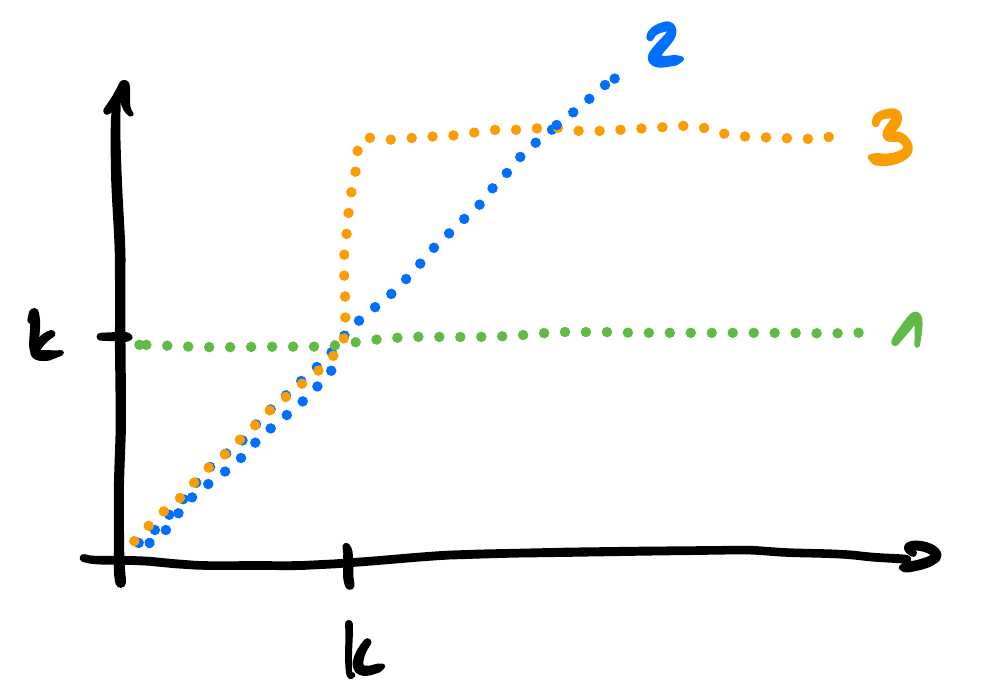
\includegraphics[width=0.3\textwidth]{images/skirental.png}
    \caption{Skirental Szenarios}
\end{figure}

\paragraph{Online-Problem}
Ein \emph{Online-Minimierungsproblem} ist $\Pi = (I, O, cost, \min)$.
Eine Eingabe $I = (x_1, ..., x_n) \in \mathcal{I}$ ist eine Folge von \emph{Anfragen},
jeweils für \emph{Zeitschritt} $i$.
Eine akzeptierte Lösung $O = (y_1, ..., y_n)$ ist eine Folge von \emph{Antworten}.

Beim analogen Maximierungsproblem spricht man statt von $cost(I, O)$ oft vom \emph{Gewinn} $gain(I,O)$.

\paragraph{Online-Algorithmus}
Sei $\Pi$ ein Online-Optimierungsproblem.
Ein \emph{Online-Algorithmus} $\A$ berechnet die Ausgabe $\A(I) = (y_1, ..., y_n) $
wobei $y_i$ nur von $(x_1, ..., x_i)$ abhängt.
$\A(I)$ ist eine zulässig Lösung für $I$.

\paragraph{Kompetitive Faktor}
(aka. competitive ratio, Wettbewerbsgüte, kompetitive Güte) \\
Ein Online-Algorithmus $\A$ ist \emph{c-kompetitiv} falls gilt:
\begin{align*}
\exists \alpha \geq 0 \quad \forall I \cl \quad cost(\A(I)) & \leq c \cdot cost(Opt(I)) + \alpha \\
\dfrac{cost(\A(I))}{cost(Opt(I))} + \alpha' & \leq c
\end{align*}
für ein Minimierungsproblem und $\alpha$ konstant.
$Opt$ ist ein optimaler Offline-Algorithmus, d.h. mit vollständiger Information.

Das kleinste $c$ für das dies gilt heisst \emph{kompetitiver Faktor}. \\
$A$ heisst \emph{strikt c-kompetitiv} falls $\alpha = 0$. \\
$\A$ heisst \emph{optimal} falls er strikt 1-kompetitiv ist ($\alpha = 0, c = 1$).

Wir sprechen hierbei von \emph{kompetitiver Analyse}.
Der kompetitiver Faktor ist vergleichbar mit der Approximationsgüte von Approximationsalgorithmen.

Ein Online-Algorithmus heisst \emph{kompetitiv} wenn sein kompetititver Faktor nicht von der
Länge der Eingabe abhängt (d.h. es keine Startkosten gibt die amortisiert werden müssen).
Die Konstante $\alpha$ ist wichtig da sie erlaubt auf kurze Eingaben schlecht zu sein
(und erst auf lange besser zu werden).
\footnote{Warum brauchen wir bei der Approximationsgüte keine vergleichbare Konstante?}

\paragraph{Untere Schranken beweisen}
Für einen strikt kompetititven Algorithmus:
Finde eine Instanz $I$ mit $\frac{\A(I)}{Opt(I)} > c$ $\implies$ \underline{nicht} strikt-kompetitiv.

Für einen nicht-strikt kompetititven Algorithmus:
Finde eine unendliche Folge $I_1, I_2, ...$ von Instanzen so dass $\frac{\A(I_i)}{Opt(I_i)} > c$
und $Opt(I_i) \overset{i \rightarrow \infty}{\longrightarrow} \infty $.

\begin{figure}[h]
    \centering
    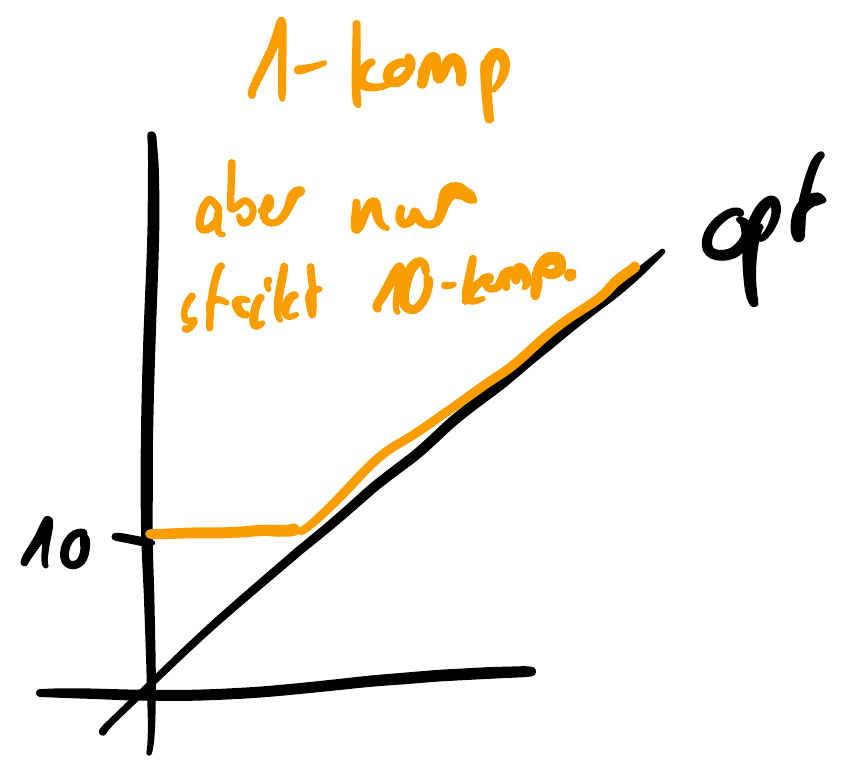
\includegraphics[width=0.2\textwidth]{images/strikt-kompetitiv.png}
    \caption{$Opt$ in schwarz. $\A$ in orange, 1-kompetitiv und strikt-10-kompetitiv.}
\end{figure}


\subsection{Das Paging-Problem}

\paragraph{Paging}
\begin{itemize}
    \item Eingabe: $ I = (x_1, ..., x_n)$ mit Speicher-Indizes $x_i \in \N$
    \item Hauptspeicher mit $m$ Seiten: $ (s_1, ..., s_m) $
    \item Cache-Speicher mit $k$ Seiten: $ B = (s_{j_1}, ..., s_{j_k}) $, initialisiert mit $ (s_1, ..., s_k) $
        \footnote{Der Vorsprung eines selbstgewählten Startinhalts kann in $\alpha$ versteckt werden.}
    \item Zeitschritt $i$:
    \begin{itemize}
        \item Index $x_i$ wird angefragt
        \item Falls $x_i$ im Cache (d.h. $s_{x_i} \in B$): return $y_i=0$
        \item Andernfalls: return $y_i=j$, und setze $B = B \backslash  \{s_j\} \cup \{s_{x_i}\} $,
            d.h. lösche Seite $s_j$ aus dem Cache.
            \footnote{Zusätzliches, proaktives Entfernen bringt keinen Vorteil.}
    \end{itemize}
    \item $ cost(\A(I)) := \vert \{ i \st y_i > 0 \} \vert $
    \item goal := min
\end{itemize}

Strategien bei \emph{Seitenfehlern (page faults)} zum \emph{Verdrängen} von Seiten:
First-in-First-Out (FIFO, wie eine Queue),
Last-in-First-Out (LIFO, wie ein Stack),
Least-Recently-Used (LRU),
Longest-Forward-Distance (LFD, offline-only!).

\paragraph{Satz}
Ein Online-Algorithmus für Paging der FIFO nutzt ist strikt-k-kompetitiv.

\underline{Beweis:}
Gruppiere Zeitschritte in \emph{Phasen}.
Phase 1 endet nach dem ersten Seitenfehler.
Phase $P \geq 2$ endet nach $1+ (P-1)k$ Seitenfehlern, d.h. alle $k$ Fehler endet eine Phase und beginnt eine neue.

In Phase 1 machen $Opt$ und $Fifo$ je genau einen Fehler (warum?).

Sei $s$ die Seite die den letzten Seitenfehler von Phase $P-1$ verursacht
(d.h. sie kommt neu in den Cache, und wird dank FIFO als letztes in Phase $P$ verdrängt werden). \\
$\implies$ Zu Beginn von Phase $P$ ist $s$ im Cache von $Opt$ \underline{und} von $Fifo$. \\
$\implies$ Es gibt $\leq k-1$ Seiten die im Cache von $Opt$ sind, aber nicht in dem von $Fifo$. \\
Während Phase $P$ macht $Fifo$ genau $k$ Fehler. \\
$\implies$  Während $P$ muss $Opt$ mindestens einen Seitenfehler machen. \\
$\implies$  $Fifo$ ist k-kompetitiv.

LRU ist in der Theorie ebenfalls k-kompetitiv, in der Praxis allerdings tendenziell besser als FIFO.


